\documentclass[]{article}
\usepackage{lmodern}
\usepackage{amssymb,amsmath}
\usepackage{ifxetex,ifluatex}
\usepackage{fixltx2e} % provides \textsubscript
\ifnum 0\ifxetex 1\fi\ifluatex 1\fi=0 % if pdftex
  \usepackage[T1]{fontenc}
  \usepackage[utf8]{inputenc}
\else % if luatex or xelatex
  \ifxetex
    \usepackage{mathspec}
    \usepackage{xltxtra,xunicode}
  \else
    \usepackage{fontspec}
  \fi
  \defaultfontfeatures{Mapping=tex-text,Scale=MatchLowercase}
  \newcommand{\euro}{€}
\fi
% use upquote if available, for straight quotes in verbatim environments
\IfFileExists{upquote.sty}{\usepackage{upquote}}{}
% use microtype if available
\IfFileExists{microtype.sty}{%
\usepackage{microtype}
\UseMicrotypeSet[protrusion]{basicmath} % disable protrusion for tt fonts
}{}
\usepackage[margin=1in]{geometry}
\usepackage{longtable,booktabs}
\usepackage{graphicx}
\makeatletter
\def\maxwidth{\ifdim\Gin@nat@width>\linewidth\linewidth\else\Gin@nat@width\fi}
\def\maxheight{\ifdim\Gin@nat@height>\textheight\textheight\else\Gin@nat@height\fi}
\makeatother
% Scale images if necessary, so that they will not overflow the page
% margins by default, and it is still possible to overwrite the defaults
% using explicit options in \includegraphics[width, height, ...]{}
\setkeys{Gin}{width=\maxwidth,height=\maxheight,keepaspectratio}
\ifxetex
  \usepackage[setpagesize=false, % page size defined by xetex
              unicode=false, % unicode breaks when used with xetex
              xetex]{hyperref}
\else
  \usepackage[unicode=true]{hyperref}
\fi
\hypersetup{breaklinks=true,
            bookmarks=true,
            pdfauthor={Abbas Rizvi},
            pdftitle={STA 546 - Homework 4},
            colorlinks=true,
            citecolor=blue,
            urlcolor=blue,
            linkcolor=magenta,
            pdfborder={0 0 0}}
\urlstyle{same}  % don't use monospace font for urls
\setlength{\parindent}{0pt}
\setlength{\parskip}{6pt plus 2pt minus 1pt}
\setlength{\emergencystretch}{3em}  % prevent overfull lines
\setcounter{secnumdepth}{0}

%%% Use protect on footnotes to avoid problems with footnotes in titles
\let\rmarkdownfootnote\footnote%
\def\footnote{\protect\rmarkdownfootnote}

%%% Change title format to be more compact
\usepackage{titling}

% Create subtitle command for use in maketitle
\newcommand{\subtitle}[1]{
  \posttitle{
    \begin{center}\large#1\end{center}
    }
}

\setlength{\droptitle}{-2em}
  \title{STA 546 - Homework 4}
  \pretitle{\vspace{\droptitle}\centering\huge}
  \posttitle{\par}
  \author{Abbas Rizvi}
  \preauthor{\centering\large\emph}
  \postauthor{\par}
  \predate{\centering\large\emph}
  \postdate{\par}
  \date{May 6, 2016}

\usepackage{subfigure}
\usepackage{graphicx}
\newcommand{\indep}{\rotatebox[origin=c]{90}{$\models$}}


\begin{document}

\maketitle


\section{Problem 1}\label{problem-1}

The \texttt{cad1} data set in the package \texttt{gRbase} was
considered. The \texttt{cad1} data set consists of 236 observations on
fourteen variables from the Danish Heart Clinic.

\subsection{Part 1A.}\label{part-1a.}

\textbf{Construct this network in R, and infer the Conditional
Probability Tables using the cad1 data. Identify any d-separations in
the graph.}

\begin{figure}[h]

{\centering 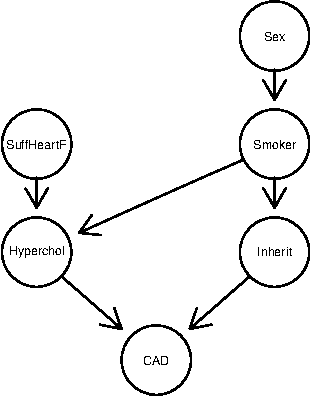
\includegraphics{stat546_hw4_files/figure-latex/unnamed-chunk-1-1} 

}

\caption{Danish Heart Clinic Network}\label{fig:unnamed-chunk-1}
\end{figure}

An `optimal network' was provided from a structural learning algorithm.
The network was recapitulated by using a directed acyclic graphical
(DAG) model (\textbf{Figure 1}). A \texttt{graph} object representing
the CAD network was created using \texttt{gRbase::dag}. The conditional
probability tables were extracted and compiled from the \texttt{graph}
by inputting the corresponding \texttt{cad1} data (\textbf{Tables 1-6})
using \texttt{gRain} functions.

The conditional probabilities that were constructed in the CAD network
\texttt{graph} object are listed below:

\begin{verbatim}
## CPTspec with probabilities:
##  P( CAD | Inherit Hyperchol )
##  P( Inherit | Smoker )
##  P( Hyperchol | SuffHeartF Smoker )
##  P( SuffHeartF )
##  P( Smoker | Sex )
##  P( Sex )
\end{verbatim}

\clearpage

D-separation was identified from the following:

\begin{align*}
1. \text{  Inheritance } &\indep \text{ Sex } \big| \text{ Smoker}\\
2. \text{  Hypercholesterolemia } &\indep \text{ Sex } \big| \text{ Smoker}\\
3. \text{  Smoker } &\indep \text{ CAD } \big| \{\text{Inheritance } \cap \text{ Hypercholesterolemia}\}\\
4. \text{  Heart Failure } &\indep \text{ CAD } \big| \text{ Hypercholesterolemia}\\
\end{align*}

\begin{table}[]
\centering
\label{my-label}
\begin{tabular}{|l|l|l|l|l|}
\hline
\multicolumn{3}{|c|}{Hypercholesterolemia = Yes}  & \multicolumn{2}{|c|}{Hypercholesterolemia = No} \\ \hline
                                    & \multicolumn{2}{|l|}{Inheritance}  &  \multicolumn{2}{|l|}{Inheritance}            \\ \hline
CAD                                 & No        & Yes & No                                 & Yes       \\ \hline
No                                  & 0.8206651 & 0.5 & 0.4488491                          & 0.2609562 \\ \hline
Yes                                 & 0.1793349 & 0.5 & 0.5511509                          & 0.7390438 \\ \hline
\end{tabular}
\caption{CAD Conditional Probability Table}
\end{table}

\begin{table}[]
\centering
\label{my-label}
\begin{tabular}{|l|l|l|}
\hline
        & \multicolumn{2}{|c|}{Smoker} \\ \hline
Inheritance & No        & Yes       \\ \hline
No      & 0.8222656 & 0.6484881 \\ \hline
Yes     & 0.1777344 & 0.3515119 \\ \hline
\end{tabular}
\caption{Genetic Inheritance Conditional Probability Table}
\end{table}

\begin{table}[]
\centering
\label{my-label}
\begin{tabular}{|r|l|l|l|l|l|}
\hline
\multicolumn{3}{|c|}{Smoker = No}                                  & \multicolumn{3}{c|}{Smoker = Yes}                                \\ \hline
\multicolumn{1}{|l|}{} & \multicolumn{2}{l|}{Suffer Heart Failure} &                      & \multicolumn{2}{l|}{Suffer Heart Failure} \\ \hline
Hypercholesterolemia   & No                  & Yes                 & Hypercholesterolemia & No                  & Yes                 \\ \hline
No                     & 0.6741294           & 0.2767857           & No                   & 0.4646226           & 0.3281787           \\ \hline
Yes                    & 0.3258706           & 0.7232143           & Yes                  & 0.5353774           & 0.6718213           \\ \hline
\end{tabular}
\caption{Hypercholesterolemia Conditional Probability Table}
\end{table}

\begin{table}[]
\centering
\label{my-label}
\begin{tabular}{|l|l|}
\hline
\multicolumn{2}{|c|}{Suffer Heart Failure}           \\ \hline
No                   & Yes       \\ \hline
0.7074513            & 0.2925487 \\ \hline
\end{tabular}
\caption{Heart Failure Conditional Probability Table}
\end{table}

\begin{table}[]
\centering
\label{my-label}
\begin{tabular}{|l|l|l|}
\hline
& \multicolumn{2}{|c|}{Sex} \\ \hline
Smoker & Female    & Male      \\ \hline
No     & 0.3622881 & 0.1802326 \\ \hline
Yes    & 0.6377119 & 0.8197674 \\ \hline
\end{tabular}
\caption{Smoker Conditional Probability Table}
\end{table}

\begin{table}[]
\centering
\label{my-label}
\begin{tabular}{|l|l|}
\hline
\multicolumn{2}{|c|}{Sex} \\ \hline
Female      & Male        \\ \hline
0.1994073   & 0.8005927   \\ \hline
\end{tabular}
\caption{Sex Conditional Probability Table}
\end{table}

\subsection{Part 1B.}\label{part-1b.}

\textbf{Suppose it is known that a new observation is female with
Hypercholesterolemia (high cholesterol). Absorb this evidence into the
graph, and revise the probabilities. How does the probability of
heart-failure and coronary artery disease (CAD) change after this
information is taken into account?}

This observation was added as evidence into our graphical model. The
output of adding the evidence was:

Given evidence that the individual is a female with
hypercholesterolemia, the probability of developing heart failure goes
from 29.2\% to 38.3\% (\textbf{Table 7}). This individual's risk of
heart failure goes up almost 10\% given her present condition.

\begin{table}[]
\centering
\begin{tabular}{|l|l|l|l|l|l|}
\hline
& \multicolumn{2}{|c|}{Heart Failure} & \multicolumn{2}{|c|}{Coronary Artery Disease} \\ \hline    
                  & No        & Yes        & No          & Yes \\ \hline
Original Evidence & 0.7074513 & 0.2925487  & 0.5401277   & 0.4598723 \\ \hline
New Evidence      & 0.6167542 & 0.3832458  & 0.3927255   & 0.6072745 \\ \hline
\end{tabular}
\caption{Old Evidence/New Evidence Conditional Probabilities of Heart Failure/CAD}
\label{my-label}
\end{table}

Likewise, when the assessing a female with hypercholesterolemia, the
probability of developing CAD increases from 45.9\% (female with no
hypercholesterolemia) to 60.7\% (female with hypercholesterolemia)
(\textbf{Table 7}).

\clearpage

\subsection{Part 1C.}\label{part-1c.}

\textbf{Simulate a new data set with new observations conditional upon this new evidence (in part B). Save this new data as a *.txt file, and submit it with your assignment. Using the new data set determine the joint distribution of “Smoker” and “CAD” given this evidence.}

A new data set was simulated (5000 simulations) with new observations
conditional upon the new evidence from part B using
\texttt{gRain::simulate.grain}. The new data set can be found in the
attached file \texttt{hw4q1c.txt}. The joint distribution of ``Smoker''
and ``CAD'' increases from 37.5\% to 42.9\% given new evidence of a
female with hypercholesterolemia (\textbf{Table 8}).

\begin{table}[]
\centering
\label{my-label}
\begin{tabular}{|l|l|l|l|l|}
\hline
       & \multicolumn{2}{|c|}{Old Evidence} & \multicolumn{2}{|c|}{Simulated New Evidence} \\ \hline
       & \multicolumn{2}{|c|}{Smoker}       & \multicolumn{2}{|c|}{Smoker} \\ \hline
CAD    & No                                 & Yes    & No     & Yes      \\ \hline
No     & 0.1320                             & 0.4081 & 0.1328 & 0.2686 \\ \hline
Yes    & 0.0845                             & 0.3754 & 0.1694 & 0.4292 \\ \hline
\end{tabular}
\caption{Joint Distribution of CAD and Smoker with Old Evidence/Simulated New Evidence}
\end{table}

\newpage 

\section{Problem 2}\label{problem-2}

The \texttt{heart.txt} data -- generated from the \texttt{reinis} data
in \texttt{gRbase library} -- was downloaded from UB Learns. The data
was collected from a 15-year follow up study of probable risk factors
for coronary thrombosis in men employed in a car factory. The variables
are: physical work, systolic blood pressure, ratio of lipoproteins,
family history of coronary heart disease. The variables systolic blood
pressure and ratio of lipoproteins are clinical markers for heart
disease.

\subsection{Part 2A.}\label{part-2a.}

The structure of the network was constructed based off of what seemed
likely and sensible in terms of variable meaning (\textbf{Figure 2}). We
constructed the model with the idea that many people who are undergoing
mental stress and physical stress at a car factory (particularly when
this study was taken place), probably smoked. Smoking can lead to high
blood pressure (systol). These individuals whom conduct mental or
physical work also may not smoke, may develop the high blood pressure
irrespective of smoking, so we designed the model so the work stress is
directly connected to high systolic blood pressure as well. Also, an
individual may have family inheritance that yields a higher
susceptibility towards having a high lipoprotein ratio, or the
individual may have family history indicating a higher susceptibility to
high blood pressure irrespective of other lipoprotein ratio -- so we
designed the model such that family history can lead to high
lipooprotein ratio and furthermore, the high lipoprotein ratio can lead
to high systolic blood pressure. A family history can also directly lead
to high systolic blood pressure.

\begin{figure}[h]

{\centering 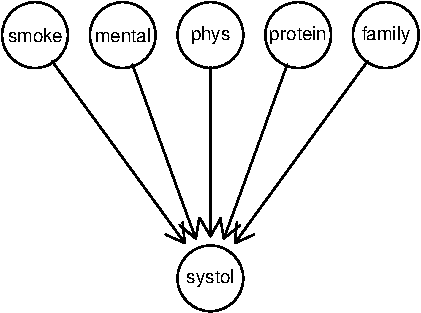
\includegraphics{stat546_hw4_files/figure-latex/unnamed-chunk-5-1} 

}

\caption{Directed Acyclic Graph of Heart.txt Variables}\label{fig:unnamed-chunk-5}
\end{figure}

\subsection{Part 2B.}\label{part-2b.}

\textbf{Based on your model in Part 2A, who is more likely to develop high systolic blood pressure (risk = yes), a person with strenuous mental work, or one with strenuous physical work, or both?}

We investigated the joint probability of an individual having high blood
pressure when there is evidence of them undergoing either physical or
mental stress alone (without evidence of the other attribute,
\textbf{Table 9}). An individual with strenuous mental work has a 33.7\%
probability of having high blood pressure and an individual with
strenuous physical work has a 29.8\% probability of having high blood
pressure (\textbf{Table 9}).

\begin{table}[]
\centering
\begin{tabular}{|l|l|l|l|l|l|}
\hline
        & \multicolumn{2}{|c|}{Mental Work} & \multicolumn{2}{|c|}{Physical Work} \\ \hline    
High Systol  & No        & Yes                & No          & Yes \\ \hline
No      & 0.1820478 & 0.2402698               & 0.2166406   & 0.205677 \\ \hline
Yes     & 0.2400985 & 0.3375839               & 0.2792904   & 0.298392 \\ \hline
\end{tabular}
\caption{Joint Probability of Mental/Physical Stress and High Systolic BP}
\label{my-label}
\end{table}

We then investigated the joint probability of individuals having high
blood pressure when there is evidence of their physical work and mental
work status (\textbf{Table 10}). When an individual does not have
strenuous physical work, but undergoes strenuous mental work during
their work day, there is a 16.2\% probability that the individual has
high blood pressure. Likewise, if an individual is undergoing both
physical and mental stress, the probability that the individual has high
blood pressure is 17.6\% (\textbf{Table 10}).

\begin{table}[]
\centering
\begin{tabular}{|l|l|l|l|l|l|}
\hline
        & \multicolumn{2}{|c|}{Physical Work = No} & \multicolumn{2}{|c|}{Physical Work = Yes} \\ \hline  
        & \multicolumn{2}{|c|}{Mental Work} & \multicolumn{2}{|c|}{Mental Work} \\ \hline    
High Systol  & No        & Yes                & No           & Yes \\ \hline
No      & 0.0918180 & 0.1248226               & 0.09022978   & 0.1154472 \\ \hline
Yes     & 0.1175374 & 0.1617530               & 0.12256107   & 0.1758309 \\ \hline
\end{tabular}
\caption{Joint Probability of High Systolic BP with Mental AND Physical Stress)}
\label{my-label}
\end{table}

Therefore, our model predicts that an individual who is experiencing
strenuous mental stress at work alone, without any evidence of their
physical work status, the probability that they are likely to develop
high blood pressure is the highest amongst all comparisons.

\clearpage

\section{Problem 3}\label{problem-3}

Webgraph A (\textbf{Figure 3}) and webgraph B (\textbf{Figure 4}) were
considered.

The PageRank matrix of the graph is defined as:

\begin{align*}
M &= (1-p) \cdot A + p \cdot B \\
\text{ where } B &= \frac{1}{n} \cdot \begin{bmatrix}
 1      & 1      & \cdots & 1\\
 \vdots & \vdots & \ddots & \vdots \\
 1      & 1      & \cdots & 1
\end{bmatrix} \\
\text{where A} &= \text{transition matrix} \\
\text{where p} &= \text{damping constant} \\
\text{where n} &= \text{number of pages}
\end{align*}

A damping factor \(p\) reflects the probability that a user who is
surfing the web quits the current page they are browsing and
``teleports'' to a new page. Damping factors are implemented in order to
overcome the problem of disconnected pages in a graph or pages with no
outgoing links.

\subsection{Part 3A}\label{part-3a}

\textbf{Compute the PageRank vector of Webgraph A for damping constants
p = 0.05, 0.25, 0.50, 0.75, and 0.95.}

\begin{figure}[h]

{\centering 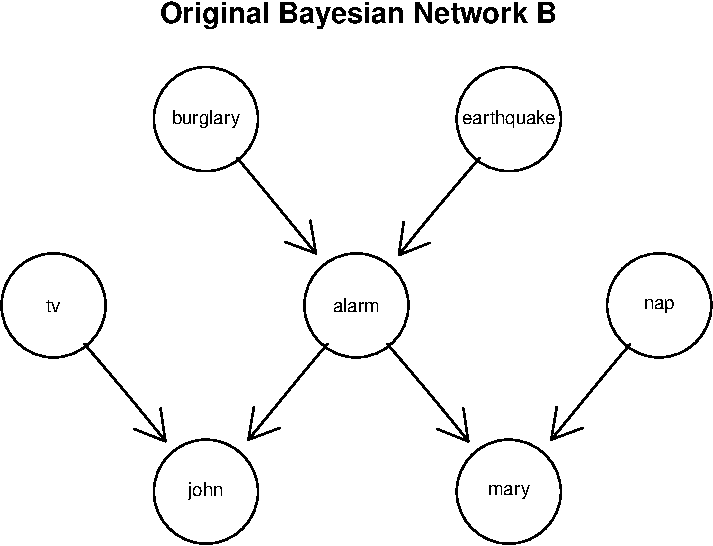
\includegraphics{stat546_hw4_files/figure-latex/unnamed-chunk-6-1} 

}

\caption{Webgraph A}\label{fig:unnamed-chunk-6}
\end{figure}

The PageRank vector for webgraph A with was computed for damping
constants \(p\) = \{0.05, 0.25, 0.50, 0.75, 0.95\} using
\texttt{igraph::page.rank}.

The highest value in the PageRank vectors
\(v_{p=0.05}, ... , v_{p=0.95}\) for webgraph A is denoted in bold type
face:

\begin{align}
v_{p=0.05}^{*} &= \begin{bmatrix}
   0.168 \\
   0.164 \\
   \bf{0.172} \\
   0.168 \\
   0.168 \\
   0.160 
 \end{bmatrix}
v_{p=0.25}^{*} &= \begin{bmatrix}
   0.179 \\
   0.154 \\
   \bf{0.185} \\
   0.176 \\
   0.173 \\
   0.132
 \end{bmatrix}
v_{p=0.50}^{*} &= \begin{bmatrix}
   \bf{0.192} \\
   0.147 \\
   0.186 \\
   0.191 \\
   0.184 \\
   0.010 
 \end{bmatrix}
v_{p=0.75}^{*} &= \begin{bmatrix}
   0.194 \\
   0.148 \\
   0.170 \\
   \bf{0.218} \\
   0.203 \\
   0.070 \\
 \end{bmatrix}
v_{p=0.95}^{*} &= \begin{bmatrix}
   0.173 \\
   0.158 \\
   0.145 \\
   \bf{0.257} \\
   0.232 \\
   0.040 \\
 \end{bmatrix}
\end{align}

\textbf{How sensitive is the PageRank vector, and overall ranking of
importance, to the damping constant? Does the relative ranking of
importance according to PageRank support your intuition?}

If we look at the equation, the greater \(p\) is, the lower the
transition matrix \(A\) is weighted and inversely, the greater \(p\) is,
more weight is given to the non-ambiguous matrix \(B\). If we look back
to the answers in \textbf{Equation (1)}, we can see that with lower
damping constants, \(p = \{0.05, 0.25\}\), the C node has the greatest
probability in the resulting PageRank vectors. Intuitively, this makes
sense, based off of the observation that C has two linking nodes and
seems to be the center of the graph. Contrarily, it seems as though when
above 0.5, the PageRank begins to converge towards node D as being the
highest PageRank in the PageRank vector. This is interesting, but it
makes sense, because as \(p\) increases to these high values, the surfer
is more likely to quit the page and ``teleport'' to a new one, and if it
starts at any of the nodes B, D, or E, there is a cycle of outgoing
links that lead back to D, so this could explain why it becomes the
highest rank in the PageRank when the \(B\) matrix holds most of the
weight.

\subsection{Part 3B}\label{part-3b}

\textbf{Compute the PageRank vector of Webgraph B for damping constant p = 0.15.}

The PageRank vector of Webgraph B (\textbf{Figure 4}) was computed with
damping constant \(p = 0.15\) using \texttt{igraph::page.rank}. The
results can be seen in \textbf{Equation (2)}.

\begin{figure}[h]

{\centering \includegraphics{stat546_hw4_files/figure-latex/3b-1} 

}

\caption{Webgraph B}\label{fig:3b}
\end{figure}

\begin{align}
v_{p=0.15}^{*} &= \begin{bmatrix}
   0.154 \\
   0.142 \\
   \bf{0.158} \\
   0.109 \\
   0.109 \\
   0.109 \\
   0.109 \\
   0.109
 \end{bmatrix} 
\end{align}

\textbf{Interpret your results in terms of the relationship between the
number of incoming links that each node has. Does the relative ranking
of importance according to PageRank support your intuition?}

The C node has the highest probability in the eigenvector \(v^{*}\) of
the \(M\) matrix for webgraph B. Intuitively, this makes sense, as 3
nodes (F, G, H) link to node C, while only two nodes link to nodes A (B
and C) and B (D and E). The PageRank probabilities of A and B seem to
reflect intuition as well, as we can see that vectors A and B have the
next two highest probabilities in the PageRank vector, which makes sense
as node A is higher than B because A linked to C (the highest PageRank).

\newpage 

\section{Problem 4}\label{problem-4}

\textbf{The sinking of the Titanic is a famous event in history. The
titanic data (UB learns) was collected by the British Board of Trade to
investigate the sinking. Many well-known facts---from the proportions of
first-class passengers to the `women and children first' policy, and the
fact that that policy was not entirely successful in saving the women
and children in the third class--- are reflected in the survival rates
for various classes of passenger. You have been petitioned to
investigate this data.}

The \texttt{titanic} data was considered. Association rules and
\textit{a priori} algorithm were implemented in order to conduct this
analysis. A support of 0.001 and confidence of 0.2 were chosen as the
minimum thresholds when setting up the rules. Support of an itemset is
defined as the proportions of transactions in the data set which contain
the item set. Confidence of a rule is defined as:
\(\frac{support(X \cap Y)}{support(X)}\).

This criteria was chosen based off of testing different numbers until
200+ rules came (and until children were represented in the item
frequency). We can see in \textbf{Figure 5} that the most represented
groups are adult, males, and non-survivors.

\begin{figure}[h]

{\centering \includegraphics{stat546_hw4_files/figure-latex/4arules-1} 

}

\caption{Item Frequency Plot of Titanic Data, Support = 0.001}\label{fig:4arules}
\end{figure}

\textbf{Summarize your findings for British Board of Trade. Is there
evidence that ``women and children'' were the first evacuated?}

We decided to subset the rules by women and children in order to
investigate this claim in the policy. We first looked at women as the
RHS of the association rules sorted by lift. We chose lift because lift
values are a solution to the problem of finding too many association
rules that satisfy the support and confidence thresholds that we set for
our analysis. A greater lift (typically \textgreater{} 1) indicates a
strong association. The results of women survivors can be seen in
\textbf{Table 11} (only showing top 5 rules).

We then looked at children survivors sorted by lift (only showing top 5
rules, \textbf{Table 12}). It seems as though children in 2nd class had
a higher probability of surviving the titanic than those from 1st class.
Just from looking at the raw data \textbf{Table 13}, we can see that
this result is probably because the sample size of children from 2nd
class is more represented than children from 1st class. We can also see
from just looking at the data (\textbf{Table 13}) that all children from
1st and 2nd class survived. And finally, our analysis reveals that the
`women and children' policy was legitimate and is supported by the
\texttt{titanic} data set.

\begin{longtable}[c]{@{}llllrrr@{}}
\caption{Association Rules with RHS = \{Survived=Yes\}, LHS =
\{Sex=Female\}}\tabularnewline
\toprule
& lhs & & rhs & support & confidence & lift\tabularnewline
\midrule
\endfirsthead
\toprule
& lhs & & rhs & support & confidence & lift\tabularnewline
\midrule
\endhead
167 & \{Class=2nd,Sex=Female,Age=Child\} & =\textgreater{} &
\{Survived=Yes\} & 0.0059064 & 1.0000000 & 3.095640\tabularnewline
99 & \{Class=1st,Sex=Female\} & =\textgreater{} & \{Survived=Yes\} &
0.0640618 & 0.9724138 & 3.010243\tabularnewline
198 & \{Class=1st,Sex=Female,Age=Adult\} & =\textgreater{} &
\{Survived=Yes\} & 0.0636075 & 0.9722222 & 3.009650\tabularnewline
84 & \{Class=2nd,Sex=Female\} & =\textgreater{} & \{Survived=Yes\} &
0.0422535 & 0.8773585 & 2.715986\tabularnewline
125 & \{Class=Crew,Sex=Female\} & =\textgreater{} & \{Survived=Yes\} &
0.0090868 & 0.8695652 & 2.691861\tabularnewline
\bottomrule
\end{longtable}

\begin{longtable}[c]{@{}llllrrr@{}}
\caption{Association Rules with RHS = \{Survived=Yes\} and LHS =
\{Age=Child\}}\tabularnewline
\toprule
& lhs & & rhs & support & confidence & lift\tabularnewline
\midrule
\endfirsthead
\toprule
& lhs & & rhs & support & confidence & lift\tabularnewline
\midrule
\endhead
62 & \{Class=2nd,Age=Child\} & =\textgreater{} & \{Survived=Yes\} &
0.0109041 & 1 & 3.09564\tabularnewline
66 & \{Class=1st,Age=Child\} & =\textgreater{} & \{Survived=Yes\} &
0.0027260 & 1 & 3.09564\tabularnewline
167 & \{Class=2nd,Sex=Female,Age=Child\} & =\textgreater{} &
\{Survived=Yes\} & 0.0059064 & 1 & 3.09564\tabularnewline
171 & \{Class=2nd,Sex=Male,Age=Child\} & =\textgreater{} &
\{Survived=Yes\} & 0.0049977 & 1 & 3.09564\tabularnewline
175 & \{Class=1st,Sex=Male,Age=Child\} & =\textgreater{} &
\{Survived=Yes\} & 0.0022717 & 1 & 3.09564\tabularnewline
\bottomrule
\end{longtable}

\begin{table}[h]
\centering
\begin{tabular}{|l|l|l|l|l|l|l|l|l|}
\hline
        & \multicolumn{4}{|c|}{Survived = No}    & \multicolumn{4}{|c|}{Survived = Yes}  \\ \hline  
        & \multicolumn{4}{|c|}{Class}            & \multicolumn{4}{|c|}{Class}           \\ \hline    
Age     & 1st & 2nd  & 3rd & Crew                & 1st & 2nd & 3rd & Crew                \\ \hline
Adult   & 122 & 167  & 476 & 673                 & 197 & 94  & 151 & 212                 \\ \hline
Child   & 0   & 0    & 52  & 0                   & 6   & 24  & 27  & 0                   \\ \hline
\end{tabular}
\caption{Survival Demographics from Raw Data Stratified by Age and Class}
\label{my-label}
\end{table}

\textbf{What characteristics/demographics are more likely in surviving passengers?}

To investigate this, we set the RHS of our association rules to
\texttt{Survived=Yes} and sorted it by lift (all rules shown,
\textbf{Table 14}). We can see from looking at the association rules in
\textbf{Table 14}, that when the RHS was \texttt{Survived=Yes}, 1st/2nd
class children were likely to survive, as well as all types of women.

\begin{longtable}[c]{@{}llllrrr@{}}
\caption{Association Rules with Survived=Yes}\tabularnewline
\toprule
& lhs & & rhs & support & confidence & lift\tabularnewline
\midrule
\endfirsthead
\toprule
& lhs & & rhs & support & confidence & lift\tabularnewline
\midrule
\endhead
62 & \{Class=2nd,Age=Child\} & =\textgreater{} & \{Survived=Yes\} &
0.0109041 & 1.0000000 & 3.095640\tabularnewline
66 & \{Class=1st,Age=Child\} & =\textgreater{} & \{Survived=Yes\} &
0.0027260 & 1.0000000 & 3.095640\tabularnewline
167 & \{Class=2nd,Sex=Female,Age=Child\} & =\textgreater{} &
\{Survived=Yes\} & 0.0059064 & 1.0000000 & 3.095640\tabularnewline
171 & \{Class=2nd,Sex=Male,Age=Child\} & =\textgreater{} &
\{Survived=Yes\} & 0.0049977 & 1.0000000 & 3.095640\tabularnewline
175 & \{Class=1st,Sex=Male,Age=Child\} & =\textgreater{} &
\{Survived=Yes\} & 0.0022717 & 1.0000000 & 3.095640\tabularnewline
99 & \{Class=1st,Sex=Female\} & =\textgreater{} & \{Survived=Yes\} &
0.0640618 & 0.9724138 & 3.010243\tabularnewline
198 & \{Class=1st,Sex=Female,Age=Adult\} & =\textgreater{} &
\{Survived=Yes\} & 0.0636075 & 0.9722222 & 3.009650\tabularnewline
84 & \{Class=2nd,Sex=Female\} & =\textgreater{} & \{Survived=Yes\} &
0.0422535 & 0.8773585 & 2.715986\tabularnewline
125 & \{Class=Crew,Sex=Female\} & =\textgreater{} & \{Survived=Yes\} &
0.0090868 & 0.8695652 & 2.691861\tabularnewline
216 & \{Class=Crew,Sex=Female,Age=Adult\} & =\textgreater{} &
\{Survived=Yes\} & 0.0090868 & 0.8695652 & 2.691861\tabularnewline
189 & \{Class=2nd,Sex=Female,Age=Adult\} & =\textgreater{} &
\{Survived=Yes\} & 0.0363471 & 0.8602151 & 2.662916\tabularnewline
127 & \{Sex=Female,Age=Adult\} & =\textgreater{} & \{Survived=Yes\} &
0.1435711 & 0.7435294 & 2.301699\tabularnewline
29 & \{Sex=Female\} & =\textgreater{} & \{Survived=Yes\} & 0.1562926 &
0.7319149 & 2.265745\tabularnewline
22 & \{Class=1st\} & =\textgreater{} & \{Survived=Yes\} & 0.0922308 &
0.6246154 & 1.933584\tabularnewline
70 & \{Sex=Female,Age=Child\} & =\textgreater{} & \{Survived=Yes\} &
0.0127215 & 0.6222222 & 1.926176\tabularnewline
108 & \{Class=1st,Age=Adult\} & =\textgreater{} & \{Survived=Yes\} &
0.0895048 & 0.6175549 & 1.911728\tabularnewline
11 & \{Age=Child\} & =\textgreater{} & \{Survived=Yes\} & 0.0258973 &
0.5229358 & 1.618821\tabularnewline
209 & \{Class=3rd,Sex=Female,Age=Adult\} & =\textgreater{} &
\{Survived=Yes\} & 0.0345298 & 0.4606061 & 1.425871\tabularnewline
116 & \{Class=3rd,Sex=Female\} & =\textgreater{} & \{Survived=Yes\} &
0.0408905 & 0.4591837 & 1.421467\tabularnewline
81 & \{Sex=Male,Age=Child\} & =\textgreater{} & \{Survived=Yes\} &
0.0131758 & 0.4531250 & 1.402712\tabularnewline
\bottomrule
\end{longtable}

\textbf{What characteristics/demographics are more likely in passengers
that perished?}

To investigate this, we set the RHS of our association rules to
\texttt{Survived=No} and sorted it by lift (all rules shown,
\textbf{Table 15}). The passengers that perished were likely to have
been men from 2nd/3rd class, crew members, and 3rd class children.

\begin{longtable}[c]{@{}llllrrr@{}}
\caption{Association Rules with Survived=No}\tabularnewline
\toprule
& lhs & & rhs & support & confidence & lift\tabularnewline
\midrule
\endfirsthead
\toprule
& lhs & & rhs & support & confidence & lift\tabularnewline
\midrule
\endhead
196 & \{Class=2nd,Sex=Male,Age=Adult\} & =\textgreater{} &
\{Survived=No\} & 0.0699682 & 0.9166667 & 1.3540828\tabularnewline
94 & \{Class=2nd,Sex=Male\} & =\textgreater{} & \{Survived=No\} &
0.0699682 & 0.8603352 & 1.2708710\tabularnewline
223 & \{Class=3rd,Sex=Male,Age=Adult\} & =\textgreater{} &
\{Survived=No\} & 0.1758292 & 0.8376623 & 1.2373791\tabularnewline
138 & \{Class=3rd,Sex=Male\} & =\textgreater{} & \{Survived=No\} &
0.1917310 & 0.8274510 & 1.2222950\tabularnewline
166 & \{Sex=Male,Age=Adult\} & =\textgreater{} & \{Survived=No\} &
0.6038164 & 0.7972406 & 1.1776688\tabularnewline
55 & \{Sex=Male\} & =\textgreater{} & \{Survived=No\} & 0.6197183 &
0.7879838 & 1.1639949\tabularnewline
156 & \{Class=Crew,Sex=Male\} & =\textgreater{} & \{Survived=No\} &
0.3044071 & 0.7772622 & 1.1481571\tabularnewline
231 & \{Class=Crew,Sex=Male,Age=Adult\} & =\textgreater{} &
\{Survived=No\} & 0.3044071 & 0.7772622 & 1.1481571\tabularnewline
48 & \{Class=Crew\} & =\textgreater{} & \{Survived=No\} & 0.3057701 &
0.7604520 & 1.1233254\tabularnewline
159 & \{Class=Crew,Age=Adult\} & =\textgreater{} & \{Survived=No\} &
0.3057701 & 0.7604520 & 1.1233254\tabularnewline
141 & \{Class=3rd,Age=Adult\} & =\textgreater{} & \{Survived=No\} &
0.2162653 & 0.7591707 & 1.1214326\tabularnewline
36 & \{Class=3rd\} & =\textgreater{} & \{Survived=No\} & 0.2398910 &
0.7478754 & 1.1047474\tabularnewline
186 & \{Class=3rd,Sex=Male,Age=Child\} & =\textgreater{} &
\{Survived=No\} & 0.0159019 & 0.7291667 & 1.0771113\tabularnewline
57 & \{Age=Adult\} & =\textgreater{} & \{Survived=No\} & 0.6533394 &
0.6873805 & 1.0153856\tabularnewline
5 & \{\} & =\textgreater{} & \{Survived=No\} & 0.6769650 & 0.6769650 &
1.0000000\tabularnewline
207 & \{Class=1st,Sex=Male,Age=Adult\} & =\textgreater{} &
\{Survived=No\} & 0.0536120 & 0.6742857 & 0.9960422\tabularnewline
76 & \{Class=3rd,Age=Child\} & =\textgreater{} & \{Survived=No\} &
0.0236256 & 0.6582278 & 0.9723218\tabularnewline
111 & \{Class=1st,Sex=Male\} & =\textgreater{} & \{Survived=No\} &
0.0536120 & 0.6555556 & 0.9683743\tabularnewline
96 & \{Class=2nd,Age=Adult\} & =\textgreater{} & \{Survived=No\} &
0.0758746 & 0.6398467 & 0.9451696\tabularnewline
17 & \{Class=2nd\} & =\textgreater{} & \{Survived=No\} & 0.0758746 &
0.5859649 & 0.8655764\tabularnewline
\bottomrule
\end{longtable}

\textbf{How do your results support the popular movie ``Titanic''? In
the movie ``Titanic'', Rose was a 1st class adult woman and survived and
Jack was 3rd class adult man and perished.}

Our association rules and analysis of the data seem to agree with this
idea from the movie (\textbf{Table 16}). The demographics that both Jack
and Rose belong to seem to agree with their respective outcomes, which
are that Jack perished and Rose survived.

\begin{longtable}[c]{@{}llllrrr@{}}
\caption{Association Rules with Jack's and Rose's
Demographics}\tabularnewline
\toprule
& lhs & & rhs & support & confidence & lift\tabularnewline
\midrule
\endfirsthead
\toprule
& lhs & & rhs & support & confidence & lift\tabularnewline
\midrule
\endhead
223 & \{Class=3rd,Sex=Male,Age=Adult\} & =\textgreater{} &
\{Survived=No\} & 0.1758292 & 0.8376623 & 1.237379\tabularnewline
198 & \{Class=1st,Sex=Female,Age=Adult\} & =\textgreater{} &
\{Survived=Yes\} & 0.0636075 & 0.9722222 & 3.009650\tabularnewline
\bottomrule
\end{longtable}

\newpage 

\section{Problem 5}\label{problem-5}

We accessed the \texttt{datasets::state} data released from the US
Department of Commerce, Bureau of the Census in R. The \texttt{state}
dataset comes with 5 assigned variables: \texttt{state.abb},
\texttt{state.area}, \texttt{state.center}, \texttt{state.division},
\texttt{state.name}, \texttt{state.region}, and \texttt{state.x77}.
\texttt{state.x77} is the raw data, while the others are factors that
may or may not be useful when clustering the data.

\subsection{Part 5A}\label{part-5a}

We decided to cluster this data in two different ways:\\1. Unsupervised
Hierarchical Clustering\\2. Principal Component Analysis

\subsubsection{Unsupervised Hierarchical
Clustering}\label{unsupervised-hierarchical-clustering}

We clustered the data in two different ways, the first being by states
(rows in the \texttt{state.x77} raw data), and the second being by state
facts (columns in the \texttt{state.x77} raw data). Hierarchical
clustering was implemented by measuring dissimilarity
(\(1 - correlation(set)\)) between observations and subsequently
computing the distance of dissimilarity (either Manhattan or Euclidean).
Furthermore, a linkage criterion (single, complete, or average linkage)
was specified to compute the pairwise distances of observations in the
sets. As this was an exploratory exercise, different combinations of
distance metrics and linkage criterion were tested, and the dendrograms
can be seen in \textbf{Figures 6-10}.

We wanted to see how well the states could cluster given the state facts
that were in the raw data. A simplified assumption of this type of
clustering is that we would expect states that are closer geographically
to one another, cluster closer together. In order to make this
quantitative method qualitative, we colored the labels by
\texttt{state.division} and \texttt{state.region}.

The labels of the dendrograms are colored by either
\texttt{state.region} or \texttt{state.divsion}. Our subjective
impression from the different clustering methods that we implemented, is
that Euclidean distance with either complete/single linkage do the best
jobs clustering this data (\textbf{Figure 6}, \textbf{Figure 7}).

\begin{figure}[h]

{\centering \includegraphics{stat546_hw4_files/figure-latex/unnamed-chunk-17-1} 

}

\caption{Heirarchical Clustering by States}\label{fig:unnamed-chunk-171}
\end{figure}\begin{figure}[h]

{\centering \includegraphics{stat546_hw4_files/figure-latex/unnamed-chunk-17-2} 

}

\caption{Heirarchical Clustering by States}\label{fig:unnamed-chunk-172}
\end{figure}\begin{figure}[h]

{\centering \includegraphics{stat546_hw4_files/figure-latex/unnamed-chunk-17-3} 

}

\caption{Heirarchical Clustering by States}\label{fig:unnamed-chunk-173}
\end{figure}

We also clustered by state facts using the same pipeline for
implementing hierarchical clustering as described above. Since there is
no way of qualitatively interpreting this data (as we do not necessarily
know any true relationships of these variables), the interpretation that
can be learned from this analysis is how different distance metrics and
linkage methods cluster the different variables and if they are
clustered near one another, the variables taken together may allow one
to predict or classify what state the data is coming from. But we can
also look at these variables with logic and make some assumptions on
which clustering method did the ``best''. However, looking at the
dendrograms in \textbf{Figure 9-10}, it seems that the different methods
mostly agree with one another. That is, the clusters are Frost-Life
Expectancy, Income-HS grad, Murder-Illiteracy, and Population-Area.

\begin{figure}[h]

{\centering \includegraphics{stat546_hw4_files/figure-latex/unnamed-chunk-18-1} 

}

\caption{Heirarchical Clustering by State Facts}\label{fig:unnamed-chunk-181}
\end{figure}\begin{figure}[h]

{\centering \includegraphics{stat546_hw4_files/figure-latex/unnamed-chunk-18-2} 

}

\caption{Heirarchical Clustering by State Facts}\label{fig:unnamed-chunk-182}
\end{figure}

\subsubsection{Principal Component
Analysis}\label{principal-component-analysis}

The second way that we looked at the relationships between the State
Fact variables was principal component analysis (PCA). This was
calculated by singular value decomposition (\texttt{stats::prcomp}) for
both of these groups, such that the data was centered and scaled. PCA is
successful if the variance of the data set is captured in the first few
PCs. We used screeplots in order to visualize how well the variance was
captured when conducting PCA by either states (\textbf{Figure 11}). We
can see that the most of the variance has been captured in the first 2
PCs (\textbf{Figure 11}).

\begin{figure}

{\centering \includegraphics{stat546_hw4_files/figure-latex/unnamed-chunk-19-1} 

}

\caption{Screeplot of PCA by States}\label{fig:unnamed-chunk-19}
\end{figure}

Next, we decided to look at biplots so we can see the dispersion of
states in the principal component space, being labeled by State Facts as
directional vectors. \textbf{Figure 12} and \textbf{Figure 13} are the
same biplots, but \textbf{Figure 12} is labeled by state region and
\textbf{Figure 13} is labeled by state division. Looking at the state
fact vectors in \textbf{Figure 12* and }Figure 13\textbf{, we can see,
visually, that the vectors that are nearest each other agree with the
clusters from the hierarchical clustering (}Figure 9, Figure 10**).
However, the biplot is more informative because we can actually see how
the states are clustering, especially when they are labeled by either
division or region. It seems as though the deep South is quite
uneducated and likely to commit murder compared to some other states. It
also seems like the colder states are generally more peaceful, survive
longer, and are more educated. It's actually quite an interesting
finding.

\begin{figure}[h]

{\centering \includegraphics{stat546_hw4_files/figure-latex/unnamed-chunk-21-1} 

}

\caption{Biplot labeled by State Regions}\label{fig:unnamed-chunk-21}
\end{figure}

\begin{figure}[h]

{\centering \includegraphics{stat546_hw4_files/figure-latex/unnamed-chunk-22-1} 

}

\caption{Biplot labeled by State Divisions}\label{fig:unnamed-chunk-22}
\end{figure}

\subsection{Part 5B}\label{part-5b}

Given the results in \textbf{Part 5A}, we were asked to develop a
Gaussian Graphical Model (GGM) from the \texttt{state} dataset and
compare our results to \textbf{5A}. GGMs are continuous graphical models
with Gaussian assumptions. We represent the data by the inverse of the
covariance matrix. The idea is impose a penalty on a sparsity which is
directly implemented from the \texttt{glasso} package in \texttt{R}. It
shrinks some of the entries of the inverse covariance matrix to 0. GGMs
should be used to describe general relationships and not as definitive
evidence of relationships. Here we implement different \(\rho\)
penalties (\(\rho=\{2, 4, 6, 10, 15, 30\}\)) to profile model
development with greater penalties (\textbf{Figure 14}). GGMs are a
reasonable way to characterize the relationship of the variables in this
dataset because they are very few variables and in these types of
situations linkage methods aren't very effective, and as such, in these
types of scenarios, graphical modeling can perhaps be the most powerful.

\begin{figure}

{\centering \includegraphics{stat546_hw4_files/figure-latex/unnamed-chunk-23-1} 

}

\caption{Gaussian Graphical Models with Different Rho Values}\label{fig:unnamed-chunk-23}
\end{figure}

We can see in \textbf{Figure 14}, that as \(\rho\) increases, the more
`less important' variables will leave the `nest'. More order begins to
come to the graphical model as \(\rho\) increases. When \(\rho\) is 10,
we see that \texttt{Frost} is quite central to the model still, but as
\(\rho\) moves to 15 and 30, \texttt{Frost} moves further down. It seems
as though for this data set, that \texttt{income} and \texttt{area} are
the central link to all of these other variables, which certainly makes
sense, because many times, the area that one lives in, dictates the cost
of living and average income of said area. Overall, it seems like we can
gather a better idea of the relationships between these state facts from
the GGM as opposed to the clustering methods used in \textbf{Part 5A}.

\end{document}
